\documentclass[notes,11pt, aspectratio=169]{beamer}

\usepackage{pgfpages}
% These slides also contain speaker notes. You can print just the slides,
% just the notes, or both, depending on the setting below. Comment out the want
% you want.
\setbeameroption{hide notes} % Only slide
%\setbeameroption{show only notes} % Only notes
%\setbeameroption{show notes on second screen=right} % Both

%\usepackage{helvet}
%\usepackage[default]{lato}
\usepackage[T1]{fontenc}
\usefonttheme{serif}
\usefonttheme{professionalfonts}
\usepackage{tgpagella}
\usepackage{array}
\usepackage{caption}
\usepackage[labelfont={color=blue}]{caption}
\usepackage{subcaption}
\usepackage{natbib}

\usepackage{tikz}
\usepackage{verbatim}
\setbeamertemplate{note page}{\pagecolor{yellow!5}\insertnote}
\usetikzlibrary{positioning}
\usetikzlibrary{snakes}
\usetikzlibrary{calc}
\usetikzlibrary{arrows}
\usetikzlibrary{decorations.markings}
\usetikzlibrary{shapes.misc}
\usetikzlibrary{matrix,shapes,arrows,fit,tikzmark}
\usepackage{amsmath}
\usepackage{mathpazo}
\usepackage{hyperref}
\usepackage{lipsum}
\usepackage{multimedia}
\usepackage{graphicx}
\usepackage{multirow}
\usepackage{graphicx}
\usepackage{dcolumn}
\usepackage{bbm}
\newcolumntype{d}[0]{D{.}{.}{5}}

\usepackage{changepage}
\usepackage{appendixnumberbeamer}
\newcommand{\beginbackup}{
   \newcounter{framenumbervorappendix}
   \setcounter{framenumbervorappendix}{\value{framenumber}}
   \setbeamertemplate{footline}
   {
     \leavevmode%
     \hline
     box{%
       \begin{beamercolorbox}[wd=\paperwidth,ht=2.25ex,dp=1ex,right]{footlinecolor}%
%         \insertframenumber  \hspace*{2ex} 
       \end{beamercolorbox}}%
     \vskip0pt%
   }
 }
\newcommand{\backupend}{
   \addtocounter{framenumbervorappendix}{-\value{framenumber}}
   \addtocounter{framenumber}{\value{framenumbervorappendix}} 
}


\usepackage{graphicx}
\usepackage[space]{grffile}
\usepackage{booktabs}

% For tables and hidding columns
\usepackage{adjustbox}
\usepackage{threeparttable}
\newcolumntype{H}{>{\setbox0=\hbox\bgroup}c<{\egroup}@{}}

\def\sym#1{\ifmmode^{#1}\else\(^{#1}\)\fi}

\usepackage{tabularx}

% These are my colors -- there are many like them, but these ones are mine.
\definecolor{blue}{RGB}{0,69,134}
\definecolor{red}{RGB}{197,0,11}
\definecolor{yellow}{RGB}{255,211,0}
\definecolor{green}{RGB}{87,157,28}

\hypersetup{
  colorlinks = true,
  linkbordercolor = {white},
  linkcolor = {blue},
  citecolor = {red}
}


%% I use a beige off white for my background
\definecolor{MyBackground}{RGB}{255,253,218}

%% Uncomment this if you want to change the background color to something else
%\setbeamercolor{background canvas}{bg=MyBackground}

%% Change the bg color to adjust your transition slide background color!
\newenvironment{transitionframe}{
  \setbeamercolor{background canvas}{bg=blue}
  \begin{frame}}{
    \end{frame}
}

\setbeamercolor{frametitle}{fg=blue}
\setbeamercolor{title}{fg=black}
\setbeamertemplate{footline}[frame number]
\setbeamertemplate{navigation symbols}{} 
\setbeamertemplate{itemize items}{-}
\setbeamercolor{itemize item}{fg=blue}
\setbeamercolor{itemize subitem}{fg=blue}
\setbeamercolor{enumerate item}{fg=blue}
\setbeamercolor{enumerate subitem}{fg=blue}
\setbeamercolor{button}{bg=MyBackground,fg=blue,}



% If you like road maps, rather than having clutter at the top, have a roadmap show up at the end of each section 
% (and after your introduction)
% Uncomment this is if you want the roadmap!
 \AtBeginSection[]
 {
    \begin{frame}
        \frametitle{Roadmap of Talk}
        \tableofcontents[currentsection]
    \end{frame}
 }
\setbeamercolor{section in toc}{fg=blue}
\setbeamercolor{subsection in toc}{fg=red}
\setbeamersize{text margin left=1em,text margin right=1em} 

% \newenvironment{itemize}{\itemize\addtolength{\itemsep}{10pt}}{\enditemize}

\usepackage{environ}
\NewEnviron{videoframe}[1]{
  \begin{frame}
    \vspace{-8pt}
    \begin{columns}[onlytextwidth, T] % align columns
      \begin{column}{.58\textwidth}
        \begin{minipage}[t][\textheight][t]
          {\dimexpr\textwidth}
          \vspace{8pt}
          \hspace{4pt} {\Large \sc \textcolor{blue}{#1}}
          \vspace{8pt}
          
          \BODY
        \end{minipage}
      \end{column}%
      \hfill%
      \begin{column}{.42\textwidth}
        \colorbox{green!20}{\begin{minipage}[t][1.2\textheight][t]
            {\dimexpr\textwidth}
            Face goes here
          \end{minipage}}
      \end{column}%
    \end{columns}
  \end{frame}
}

\title[]{\textcolor{blue}{The Effect of Information on Wages: Evidence from the IMSS RPCI in Mexico}}
\author[Marco Medina]{Marco Medina}
\date{November 23, 2023}


\begin{document}

%%% TIKZ STUFF
\tikzset{   
        every picture/.style={remember picture,baseline},
        every node/.style={anchor=base,align=center,outer sep=1.5pt},
        every path/.style={thick},
        }
\newcommand\marktopleft[1]{%
    \tikz[overlay,remember picture] 
        \node (marker-#1-a) at (-.3em,.3em) {};%
}
\newcommand\markbottomright[2]{%
    \tikz[overlay,remember picture] 
        \node (marker-#1-b) at (0em,0em) {};%
}
\tikzstyle{every picture}+=[remember picture] 
\tikzstyle{mybox} =[draw=black, very thick, rectangle, inner sep=10pt, inner ysep=20pt]
\tikzstyle{fancytitle} =[draw=black,fill=red, text=white]
%%%% END TIKZ STUFF

% Title Slide
\begin{frame}
\maketitle
  % \centering The views expressed do not necessarily reflect the position of Somewhere Fancy.
\end{frame}

\section{Motivation}
\begin{transitionframe}
  \begin{center}
    \Huge \textcolor{white}{Motivation}
  \end{center}
\end{transitionframe}


\begin{frame}[fragile]{Motivation}
  \begin{itemize}[<+->]
    \vfill\item Payroll tax evasion manifests along various dimensions:
    \begin{itemize}
        \vfill\item Firms not registering with the tax authorities (\textcolor{red}{extensive margin}).
        \vfill\item Workers hired without being reported to tax authorities (\textcolor{red}{intensive margin}).
    \end{itemize}
    \vfill\item Most research focuses on the first two. \citep{Ulyssea}. This work focuses on a third margin.
    \begin{itemize}
        \vfill\item Workers reported to tax authorities with lower wages than they actually receive (\textcolor{red}{intra-intensive margin}). \citep{kumler2020enlisting}.
        \vfill\item Inspections can increase monthly wages but are costly and can decrease formal employment. \citep{samaniego2020increasing}
        \vfill\item Self-enforcing mechanisms like information can improve reporting while being a low-cost solution compared to inspections.
    \end{itemize}
    \end{itemize}
\end{frame}


\begin{frame}
\frametitle{Motivation}
\begin{itemize}[<+->]
    \vfill\item<1-> In Mexico, employers report the wages of formal workers to IMSS (Mexican Social Security Institute).
    \begin{itemize}
        \vfill\item<2-> Some employers underreport wages to pay less in employer contributions and taxes.
        \vfill\item<3-> Underreporting decreases the benefits for the worker (pension, AFORE retirement savings, disability insurance, etc.)
    \end{itemize}
    \vfill\item<4-> Underreporting can be either agreed upon or not.
    \begin{itemize}
        \vfill\item<5-> There might be an agreement to share the tax savings between employer and employee.
        \vfill\item<6-> The employer might underreport without the knowledge of the employee.
    \end{itemize}
\end{itemize}
\end{frame}


\begin{frame}
\frametitle{Motivation}
\begin{itemize}[<+->]
    \vfill\item<1-> How much do workers know about their reported wages and current enrollment?
    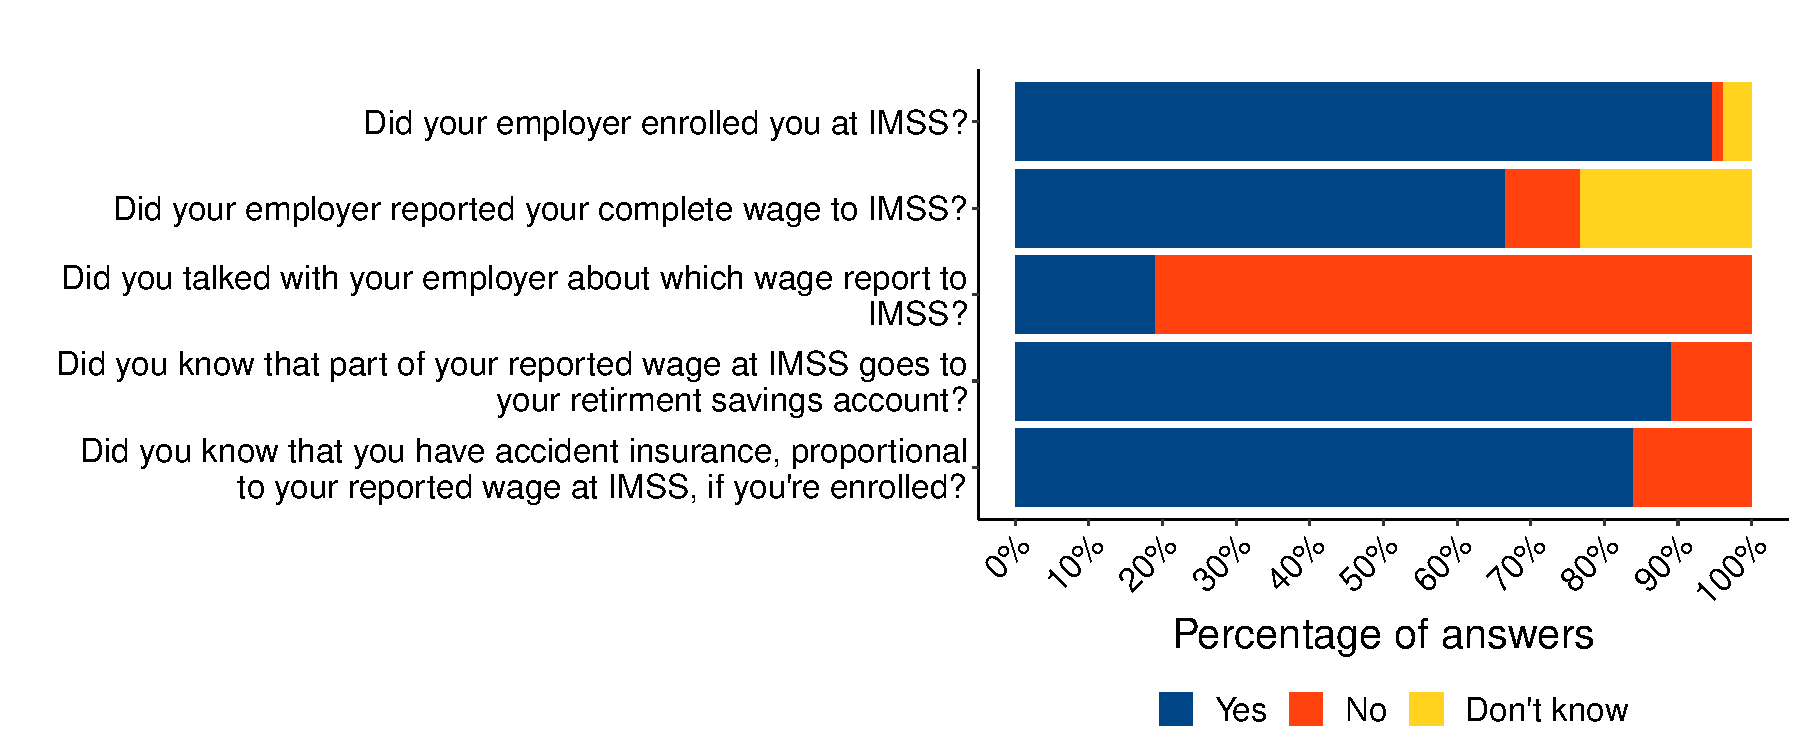
\includegraphics[width=0.9\textwidth]{04_Figures/worker_survey/hist_knowledge_register_survey.pdf}
\end{itemize}
\end{frame}


\section{RPCI}
\begin{transitionframe}
  \begin{center}
    \Huge \textcolor{white}{RPCI}
  \end{center}
\end{transitionframe}


\begin{frame}
\frametitle{RPCI}
\begin{itemize}[<+->]
    \vfill\item<1-> When can workers identify underreporting?
    \begin{itemize}
        \vfill\item<2-> When approaching retirement, through their IMSS reported contribution weeks.
        \vfill\item<2-> Incorrectly reported wages are difficult to correct.
        \begin{itemize}
            \vfill\item<3-> Lack of receipts to prove the correct wages.
            \vfill\item<3-> The employing companies might no longer exist.
        \end{itemize}
    \end{itemize}
    \vfill\item<4-> \textbf{RPCI (Reporte Personalizado de Cotización en el IMSS)}
    \begin{itemize}
        \vfill\item<5-> A report for the worker with the employer's business name and their reported wage.
        \vfill\item<6-> Workers sign up once and receive the report month by month.
    \end{itemize}
\end{itemize}
\end{frame}


\begin{frame}{RPCI Example}
    \begin{figure}[H]
    \label{rpci_example}
    \begin{center}
    
    \begin{subfigure}{0.49\textwidth}
    \caption{RPCI within the IMSS Digital app}
    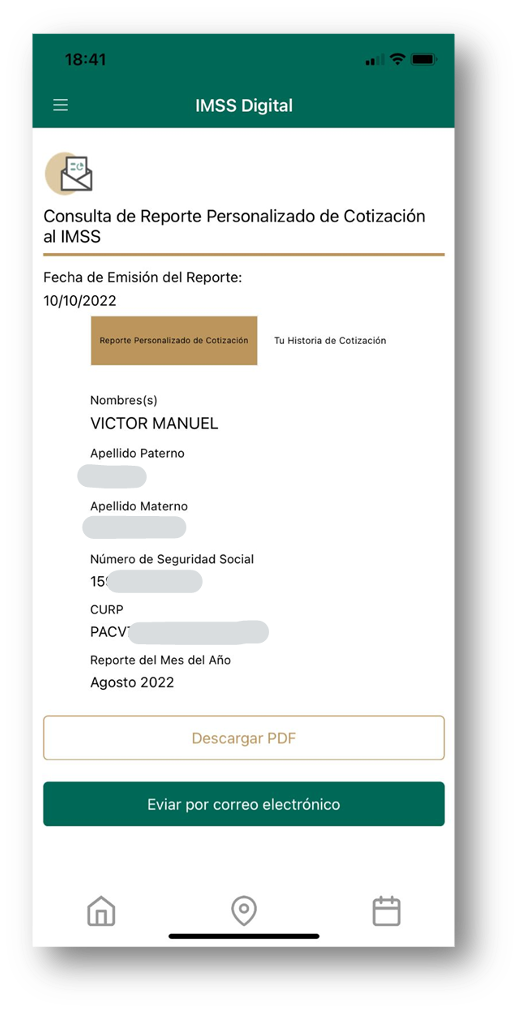
\includegraphics[width=\textwidth]{04_Figures/rpci_app/rpci_2.png}
    \end{subfigure}
    \begin{subfigure}{0.49\textwidth}
    \caption{RPCI PDF file}
    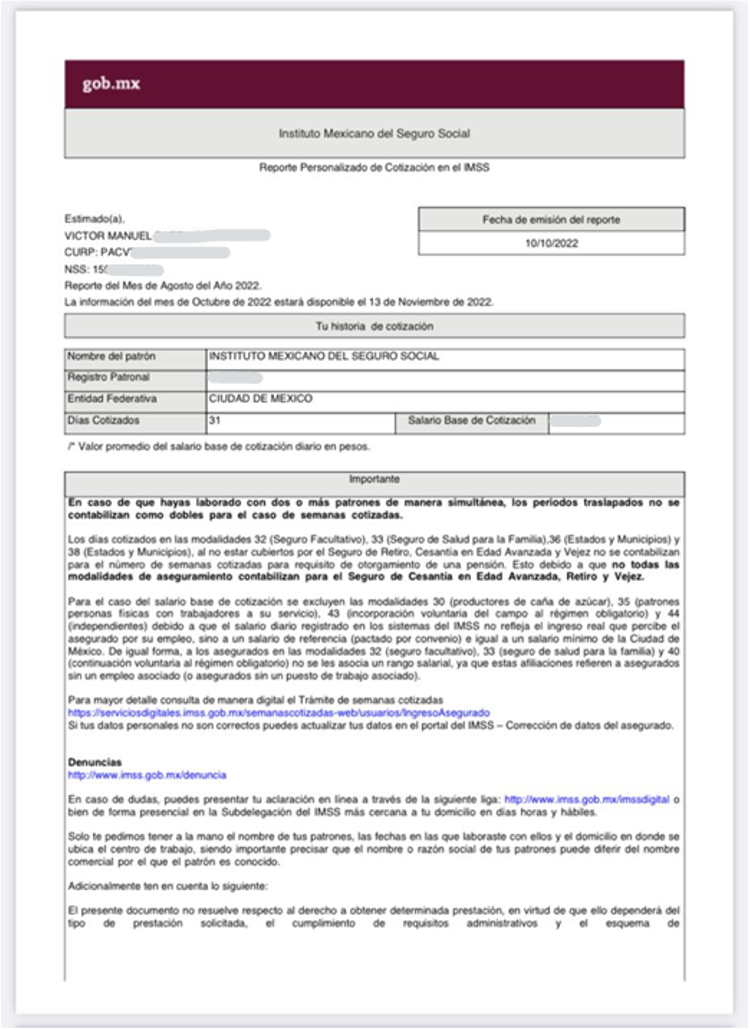
\includegraphics[width=\textwidth]{04_Figures/rpci_app/rpci_3.png}
    \end{subfigure}

    \end{center}
\end{figure}
\end{frame}

\section{Data}
\begin{transitionframe}
  \begin{center}
    \Huge \textcolor{white}{Data}
  \end{center}
\end{transitionframe}

\begin{frame}
\frametitle{Administrative Data from IMSS}
\begin{itemize}
    \vfill\item Monthly panel dataset for a random sample of workers registered at IMSS during 2020 and January 2021, one month before the RPCI launch.
    \vfill\item The dataset tracks workers from January 2018 to February 2022, including information on their wage, industry, age group, firm, job modality, state, and RPCI registration.
\end{itemize}

\vfill
\begin{block}{Summary Statistics}
    \begin{itemize}
        \item Over 1,400,000 workers and 339,000 firms observed.
        \item 39\% women, 21\% in outsourcing, 10\% eventual workers.
        \item Average daily wage: $\$492.44$ MXN (approx. $\$25$ USD in February 2021).
    \end{itemize}
\end{block}
\end{frame}

\section{Specification}
\begin{transitionframe}
  \begin{center}
    \Huge \textcolor{white}{Specification}
  \end{center}
\end{transitionframe}

\begin{frame}
\frametitle{Specification}
\begin{itemize}
    \vfill\item Our main analysis uses panel data, with the treatment being registration for the RPCI.
    \vfill\item \textbf{Staggered treatment design:} Workers can register for RPCI anytime after its launch and receive the reports each month.
    \vfill\item We observed different treatment cohorts monthly since RPCI's launch, with a pure control group comprising workers who never registered for RPCI.
    \vfill\item We employ a DID approach accounting for possible heterogeneous effects across cohorts.
\end{itemize}
\end{frame}

\begin{frame}{Difference-in-Difference (DID) Analysis}
    \begin{itemize}
        \vfill\item Initial approach: Two-way fixed effects (TWFE) specification.
        \vfill\item Addressing TWFE limitations: Recent literature (\citealt{de2020two}; \citealt{callaway2021difference}; \citealt{sun2021estimating}) highlights potential biases in TWFE due to heterogeneous treatment effects.
        \vfill\item Alternative specification: We employ the method proposed by \cite{de2020two} for robust dynamic analysis, suited for large samples and accounting for heterogeneous effects across cohorts.
    \end{itemize}

    \vfill
    \textit{Note: Other estimators like \cite{callaway2021difference} and \cite{sun2021estimating} are computationally challenging for large samples.}
\end{frame}

\section{Results}
\begin{transitionframe}
  \begin{center}
    \Huge \textcolor{white}{Results}
  \end{center}
\end{transitionframe}

\begin{frame}{Event studies of the effect on enrollment and wages}

\begin{figure}[H]
    \centering
    %\caption{Event studies - RPCI effect on enrollment and wages \label{fig:event_study_rpci}}
    
    \begin{subfigure}{0.38\textwidth}
    \caption{Effect on being enrolled}
    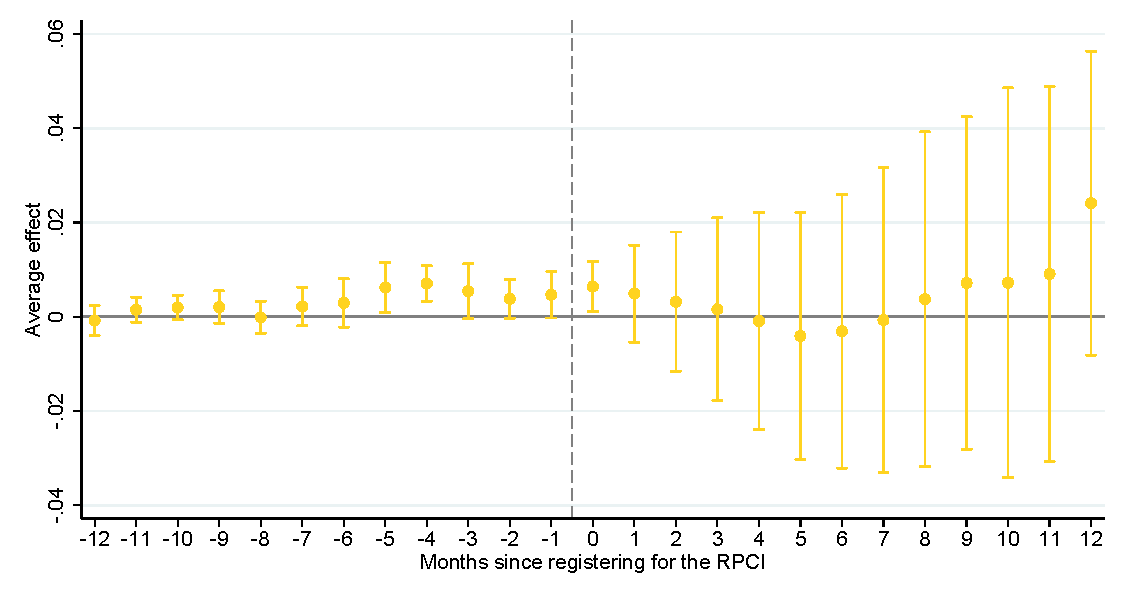
\includegraphics[width=\textwidth]{04_Figures/muestra_10porciento/event_study_alta_dcdh.pdf}
    \end{subfigure}
    \begin{subfigure}{0.38\textwidth}
    \caption{Effect on formal wage$^\dagger$}
    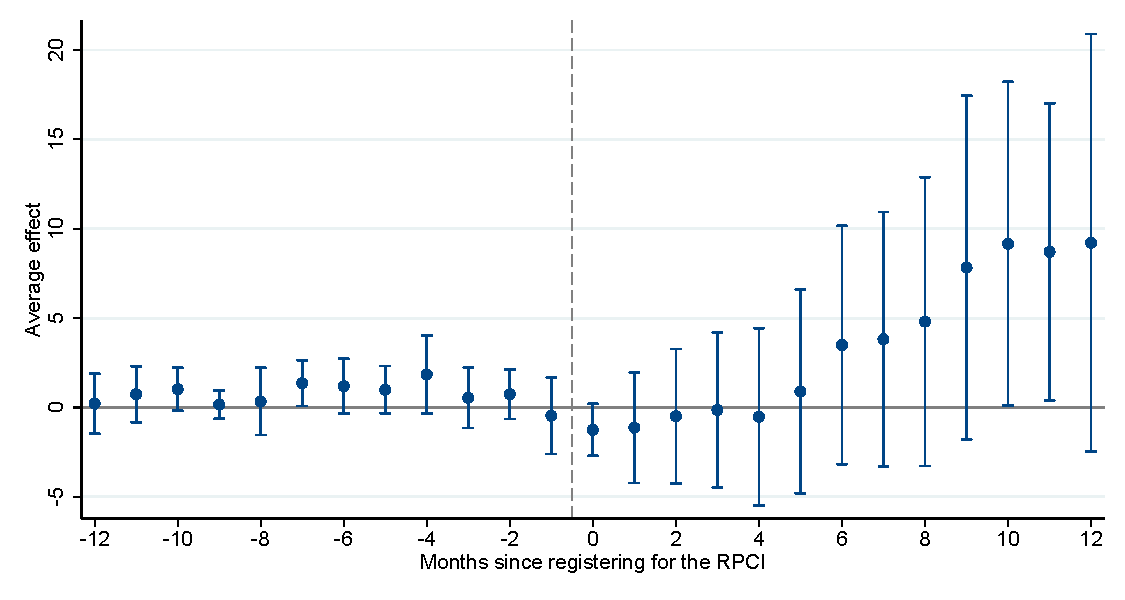
\includegraphics[width=\textwidth]{04_Figures/muestra_10porciento/event_study_sal_formal_dcdh.pdf}
    \end{subfigure}
    
    \begin{subfigure}{0.38\textwidth}
    \caption{Effect on wage}
    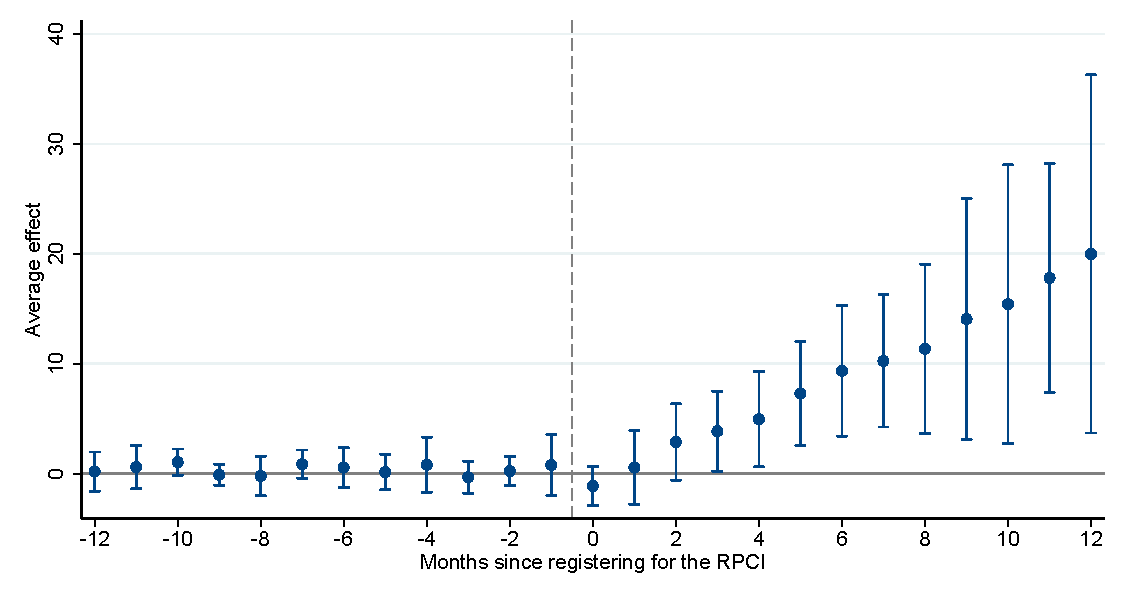
\includegraphics[width=\textwidth]{04_Figures/muestra_10porciento/event_study_sal_cierre_dcdh.pdf}
    \end{subfigure}
    \begin{subfigure}{0.38\textwidth}
    \caption{Effect on log wage}
    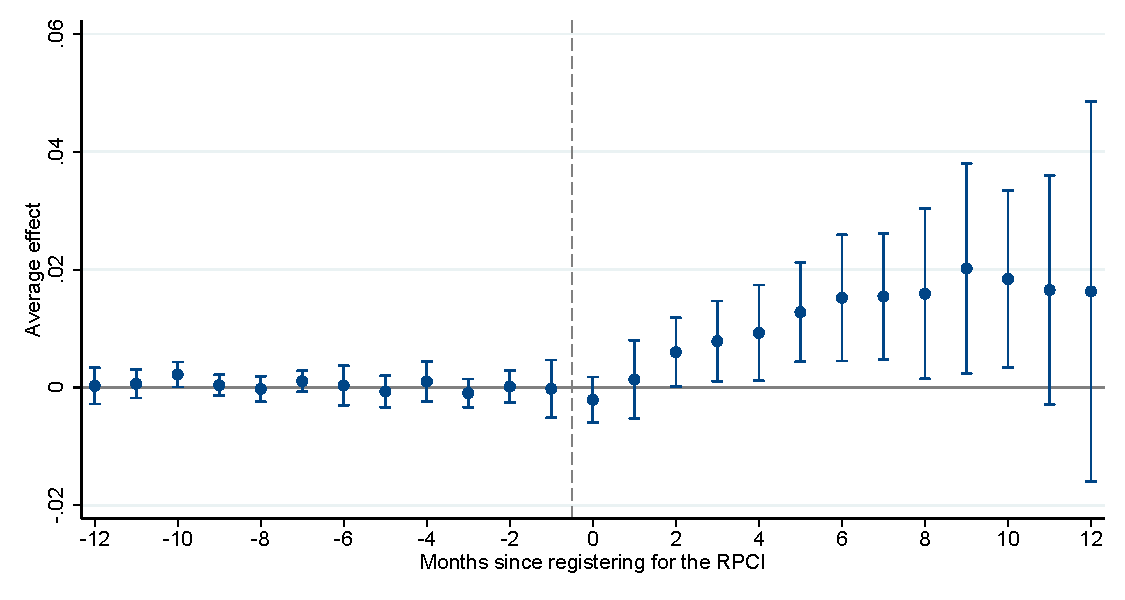
\includegraphics[width=\textwidth]{04_Figures/muestra_10porciento/event_study_log_sal_cierre_dcdh.pdf}
    \end{subfigure}
    
    %\textit{Do file: event_study_rpci.do}
\end{figure}
    
\end{frame}

\begin{frame}[fragile]{RPCI effect on enrollment and wages}
\begin{table}[H]
\footnotesize
\centering
\begin{threeparttable}
\centering
%\caption{RPCI effect on enrollment and wages\label{tab:dcdh_rpci}}
%\textit{Do file: event_study_rpci.do}

\begin{tabular}[t]{@{}l@{}l@{}l@{}l}
\toprule
\toprule
\multicolumn{4}{c}{ATE using \cite{de2020two}} \\
\midrule
\begin{tabular}[t]{lc}
& Enrolled \\
\midrule
\input 03_Tables/muestra_10porciento/dcdh_alta
\end{tabular}
&
\begin{tabular}[t]{Hc}
& Formal Wage$^\dagger$ \\
\midrule
\input 03_Tables/muestra_10porciento/dcdh_sal_formal
\end{tabular}
&
\begin{tabular}[t]{Hc}
& Wage \\
\midrule
\input 03_Tables/muestra_10porciento/dcdh_sal_cierre
\end{tabular}
&
\begin{tabular}[t]{Hc}
& Log Wage \\
\midrule
\input 03_Tables/muestra_10porciento/dcdh_log_sal_cierre
\end{tabular}

\tabularnewline 
\bottomrule
\bottomrule

\end{tabular}
\end{threeparttable}
\end{table}
\end{frame}

\begin{frame}[fragile]{Heterogeneity by worker characteristics}
\begin{figure}[H]
    \centering
    %\caption{Heterogeneity by worker characteristics \label{fig:heterogeneity_worker_rpci}}
    
    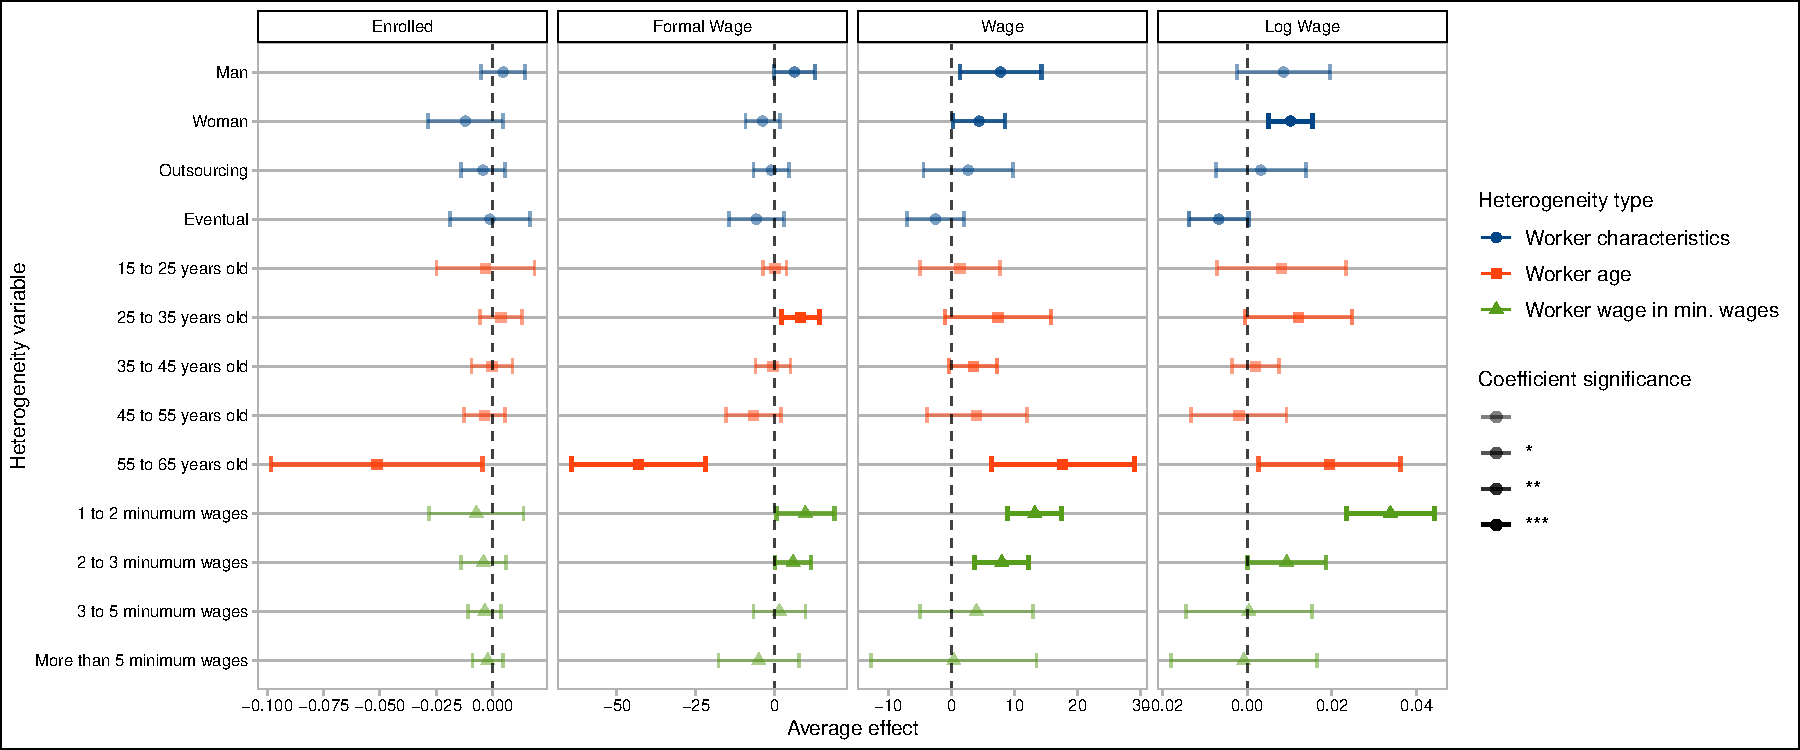
\includegraphics[width=\textwidth]{04_Figures/muestra_10porciento/dcdh_heterogeneity_worker_characteristics.pdf}
    
    %\textit{Do file: dcdh_heterogeneity_rpci.do}
\end{figure}
\end{frame}

\begin{frame}[fragile]{Heterogeneity by firm characteristics}
\begin{figure}[H]
    \centering
    %\caption{Heterogeneity by firm characteristics \label{fig:heterogeneity_firm_rpci}}
    
    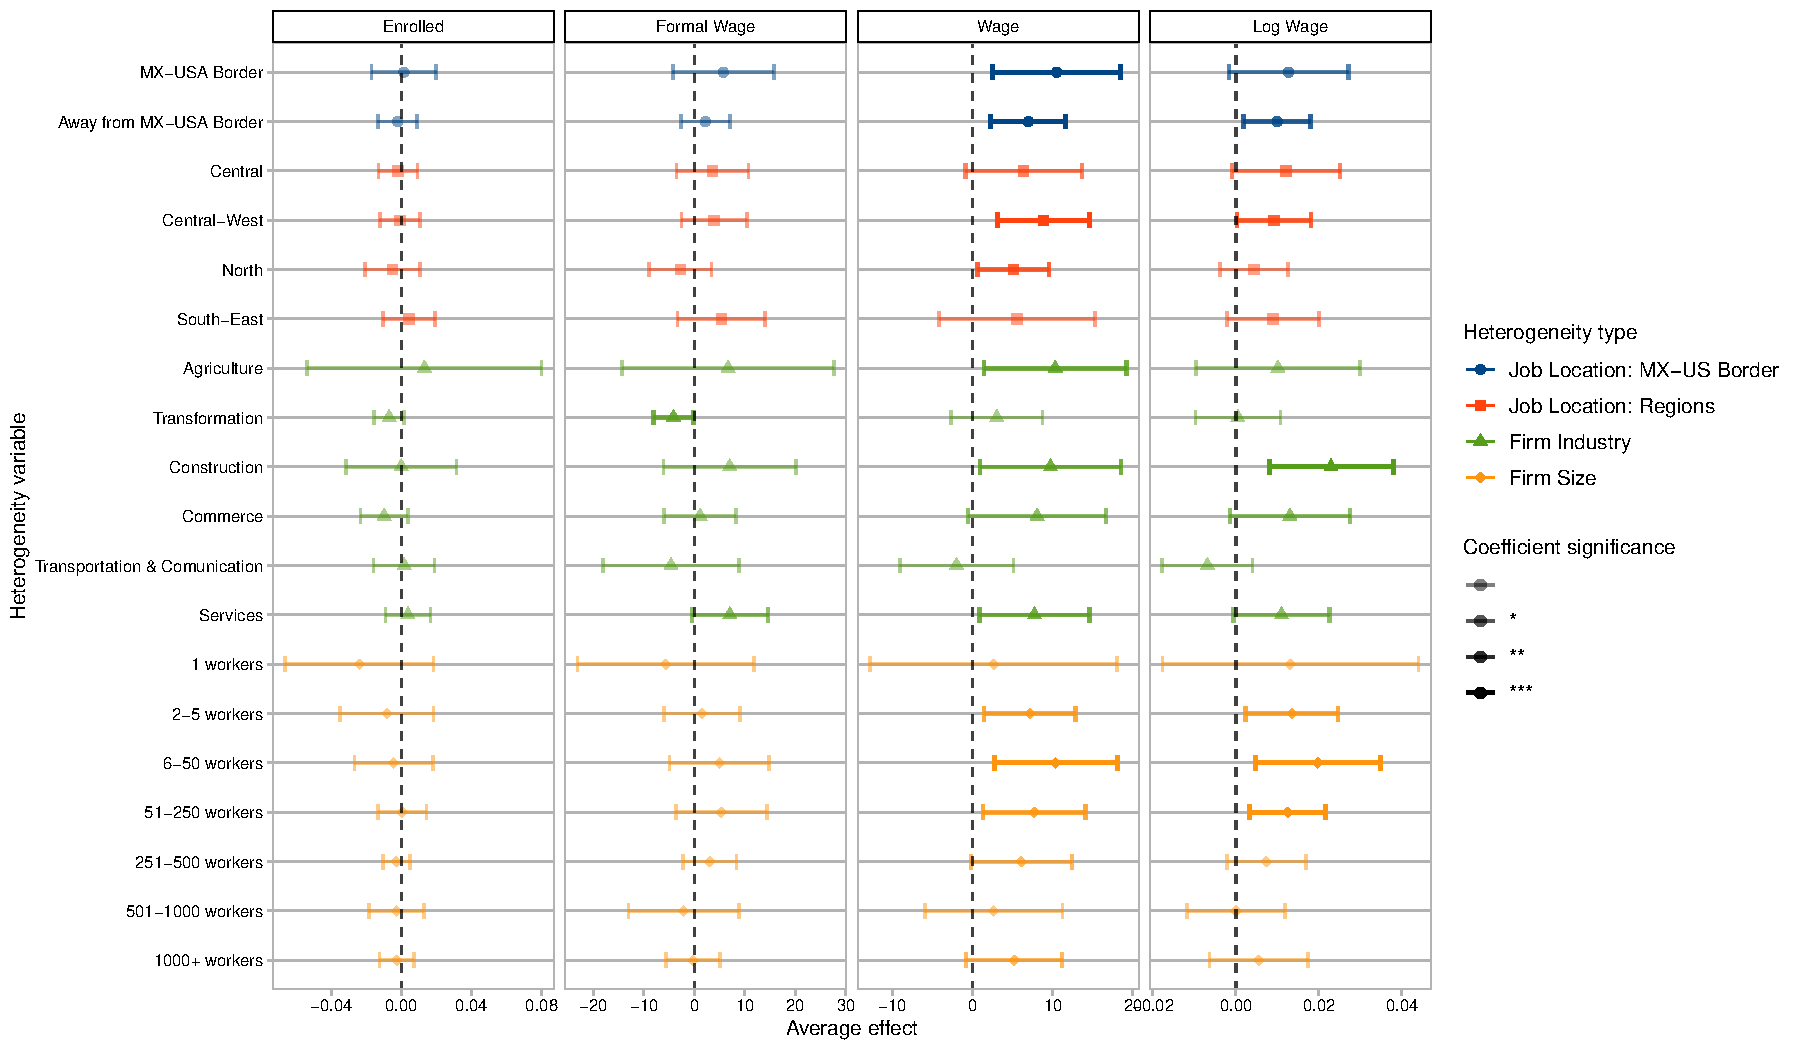
\includegraphics[width=0.95\textwidth]{04_Figures/muestra_10porciento/dcdh_heterogeneity_firm_characteristics.pdf}
    
    %\textit{Do file: dcdh_heterogeneity_rpci.do}
\end{figure}
\end{frame}

\begin{frame}{Heterogeneity Summary}
\begin{itemize}
    \vfill\item The effect on wages is bigger for men that women in absolute terms, but bigger for women in relative terms.
    \vfill\item There is a negative effect on enrollment for people near retirement age, but a big and positive effect on wages. \textit{Make or break negotiation?}
    \vfill\item The effect is bigger for workers earning near the minimum (an average effect of 18\% the minimum wage in 2021).
    \vfill\item The effect is bigger for workers registered at small and medium firms.
\end{itemize}
    
\end{frame}

\section{Mechanisms?}
\begin{transitionframe}
  \begin{center}
    \Huge \textcolor{white}{Mechanisms?}
  \end{center}
\end{transitionframe}

\begin{frame}{RPCI effect on filing lawsuits in the MCLC}
\begin{itemize}
    \vfill\item IMSS matched data with lawsuits filed at the Mexico City Labor Court between 2020 and 2022.
    \vfill\item There is a treatment effect one month after that is three times the variable mean.
    \vfill\item \textit{Does wage increases are via lawsuits?}

    \begin{figure}[H]
    \centering
    
    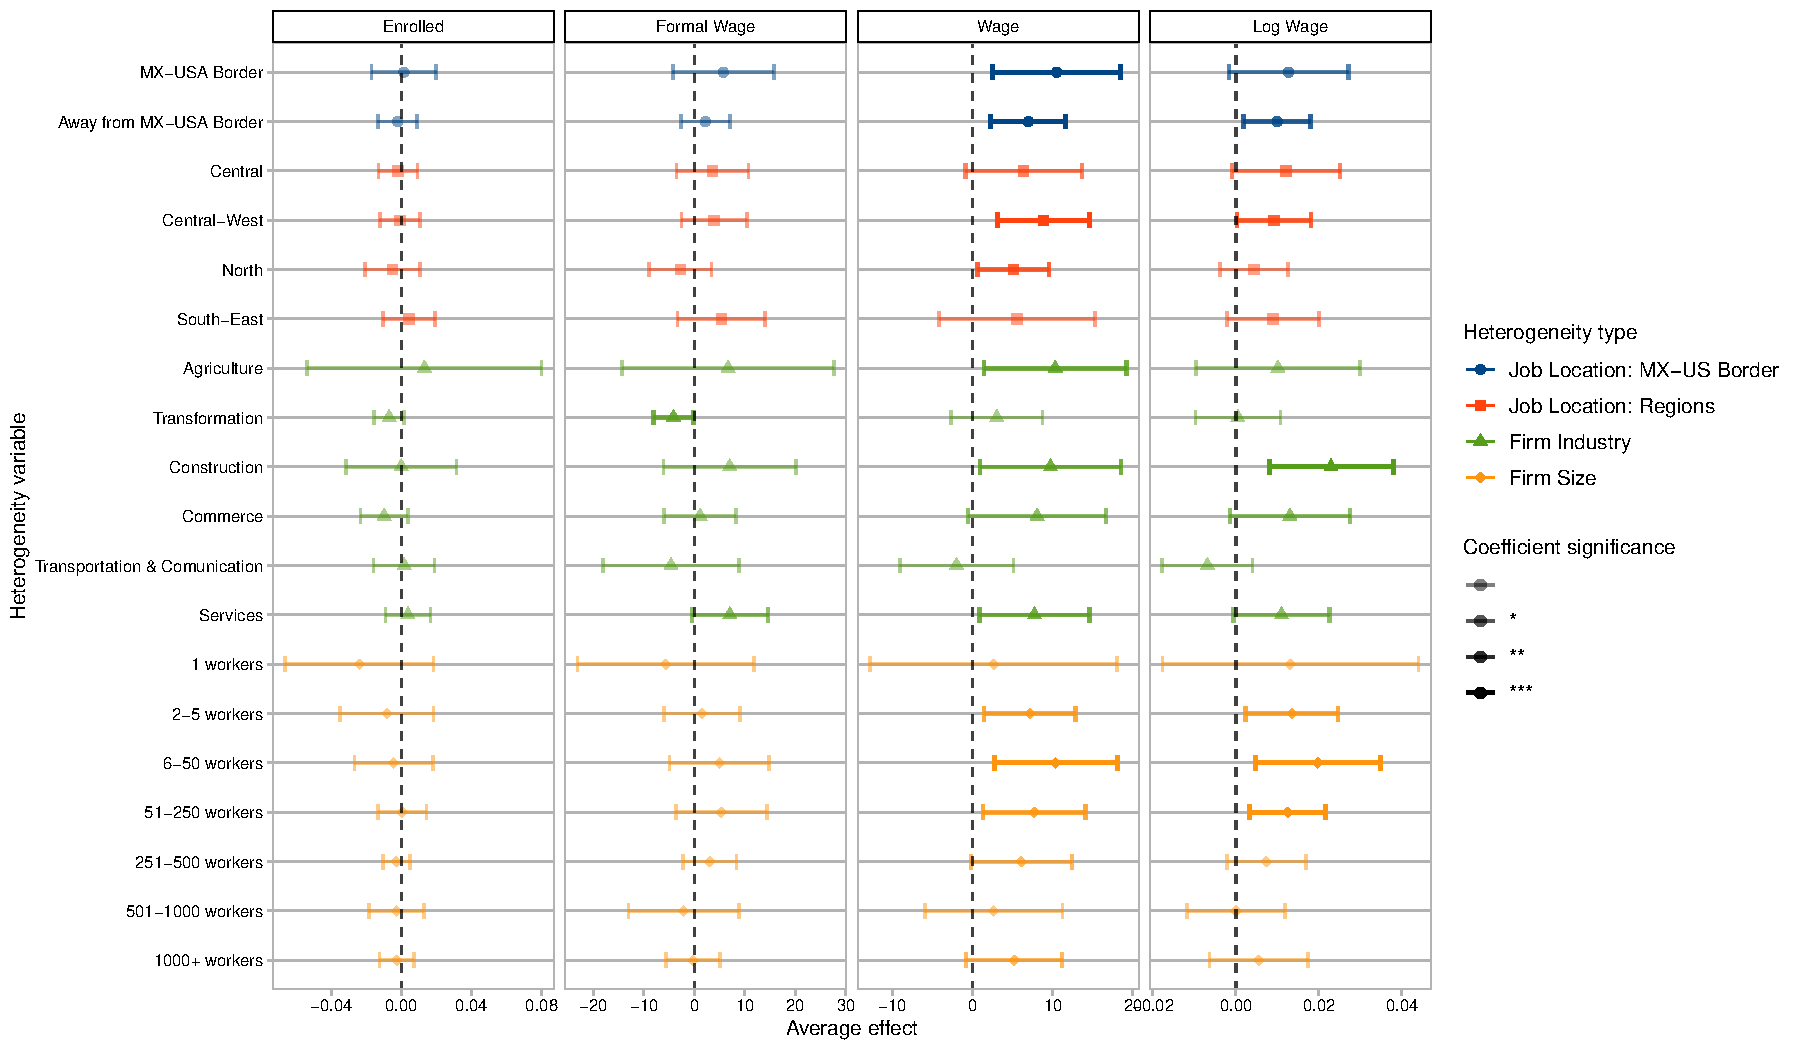
\includegraphics[width=0.95\textwidth]{04_Figures/muestra_10porciento/dcdh_heterogeneity_firm_characteristics.pdf}
    
    \end{figure}

\end{itemize}
    
\end{frame}



\begin{frame}[plain]{Thanks :)}
\begin{itemize}
 \item Questions? Thoughts? Comments?
\end{itemize}
\end{frame}


\section{References}
\begin{frame}[allowframebreaks]{References}
\bibliographystyle{ecta}
\bibliography{05_Report/02_Tesis/References}
\end{frame}

\section{Appendix}
\begin{transitionframe}
  \begin{center}
    \Huge \textcolor{white}{Appendix}
  \end{center}
\end{transitionframe}

\end{document}